% Afficher des recommendations concernant la syntaxe.
\RequirePackage[orthodox,l2tabu]{nag}
\RequirePackage{luatex85}
% Paramètres du document.
\documentclass[%
a3paper%                       Taille de page.
,fontsize=47pt%                Taille de police.
,DIV=17%                       Plus grand => des marges plus petites.
,titlepage=off%                Faut-il une page de titre ?
,headings=optiontoheadandtoc%  Effet des paramètres optionnels de section.
,headings=small%
,parskip=false%
,openany%
]{scrbook}
\renewcommand*\partheademptypage{\thispagestyle{empty}}

%\usepackage{geometry}

% Par souci de clarté, la définition des commandes est reportée dans un document annexe.
\usepackage{gredoc,mudoc,lyluatex}
\usepackage{pdfpages,transparent,array,ltablex}
\addtolength{\voffset}{2mm}\addtolength{\headsep}{-2mm}
\setlength{\extrarowheight}{2mm}
\addto\captionsfrench{%
  \renewcommand{\indexname}{Index des chants}%
}

\pdfcompresslevel=9

\newcommand{\lieu}[1]{\hfill\linebreak[3]\hspace*{\stretch{1}}\nolinebreak\mbox{\emph{(#1)}}}

\newcommand{\commandement}[1]{\noindent\textbf{#1}}

\newcommand{\schola}[1]{}\newcommand{\foule}[1]{#1}
\providecommand{\dest}{foule}

\newcommand{\bgimage}[1]{%
\raisebox{-.45\paperheight}[0pt][0pt]{%
  \transparent{0.3}%
  \includegraphics[width=.7\paperwidth,height=.7\paperheight,keepaspectratio=true]{img/#1}%
  }%
}

\def\arraystretch{1.2}


\grechangedim{overhepisemalowshift}{.7mm}{scalable}
\grechangedim{hepisemamiddleshift}{1.4mm}{scalable}
\grechangedim{overhepisemahighshift}{2.1mm}{scalable}
\grechangedim{vepisemahighshift}{2.1mm}{scalable}

\title{Cantus}
\date{}

\def\blindsection#1{\markright{#1}\addcontentsline{toc}{section}{#1}}

%\pagestyle{empty}

%\includeonly{Parties/Kyriale-XI}

\begin{document}

\thispagestyle{empty}

%{\centering \textbf{Kyriale I}\par}

\bigskip

\cantus{Kyriale}{Kyrie-I}{}{8.}

\cantus{Kyriale}{Gloria-I}{}{4.}

\cantus{Kyriale}{Sanctus-I}{}{4.}

\cantus{Kyriale}{Agnus-I}{}{4.}

%\cantus{Kyriale}{Ite-XI}{}{1.}

%{\centering \textbf{Kyriale II}\par}

\bigskip

\cantus{Kyriale}{Kyrie-II}{}{3.}

\cantus{Kyriale}{Gloria-II}{}{1.}

\cantus{Kyriale}{Sanctus-II}{}{1.}

\cantus{Kyriale}{Agnus-II}{}{1.}

%\cantus{Kyriale}{Ite-XI}{}{1.}

%{\centering \textbf{Kyriale IV}\par}

\bigskip

\cantus{Kyriale}{Kyrie-IV}{}{1.}

\cantus{Kyriale}{Gloria-IV}{}{4.}

\cantus{Kyriale}{Sanctus-IV}{}{8.}

\cantus{Kyriale}{Agnus-IV}{}{6.}

%{\centering \textbf{Kyriale XI}\par}

\bigskip

\cantus{Kyriale}{Kyrie-XI}{}{1.}

\pagebreak[3]
\cantus{Kyriale}{Gloria-XI}{}{2.}

{%
\grechangedim{spacelinestext}{2.8ex}{scalable}
\cantus{Kyriale}{Sanctus-XI}{}{2.}

\grechangedim{spaceabovelines}{1.5ex}{scalable}
\cantus{Kyriale}{Agnus-XI}{}{1.}%
}

%\cantus{Kyriale}{Ite-XI}{}{1.}

%{\centering \textbf{Credo I}\par}

\bigskip

\cantus{Kyriale}{Credo-I}{}{4.}

%{\centering \textbf{Feria VI.\\Quatuor Temporum Adventus}\par}

\bigskip


\cantus{Introit}{PropeEsTu}{Intr.}{4.}

\cantus{Graduel}{OstendeNobis}{Grad.}{2.}

\cantus{Offertoire}{DeusTuConvertens}{Off.}{4.}

\cantus{Communion}{EcceDominusVeniet}{Comm.}{6.}

%{\centering \textbf{In Epiphania Domini}\par}

\bigskip

{%
\gresetinitiallines{2}
\greillumination{\raisebox{2ex}{\hspace{-1ex}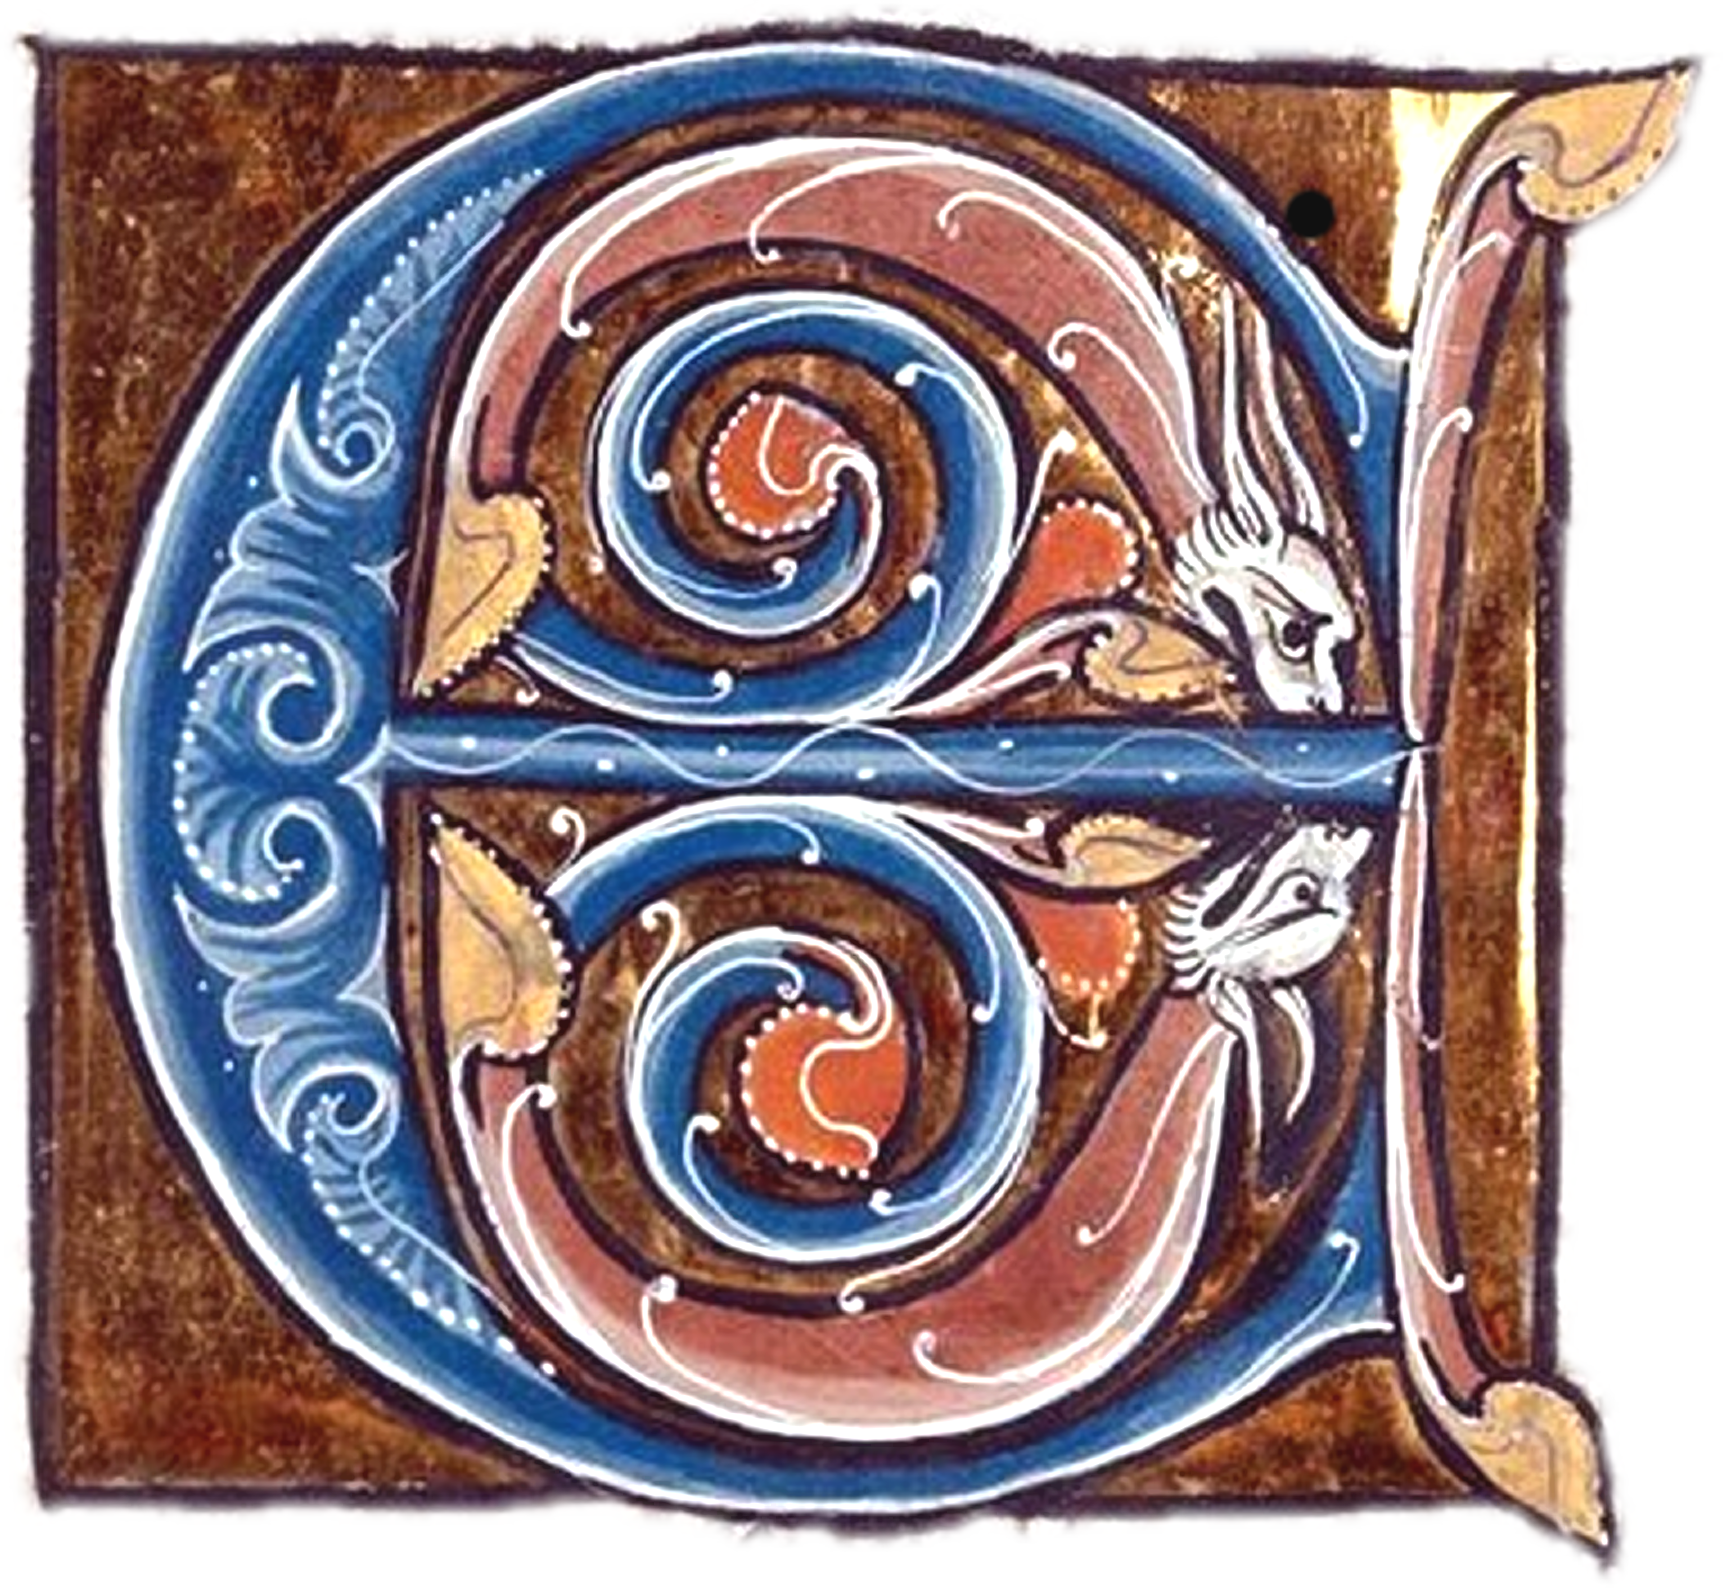
\includegraphics[height=12ex]{img/E0001}}}
\cantus{Introit}{EcceAdvenit}{Intr.}{2.}%
}

\cantus{Graduel}{OmnesDeSaba}{Grad.}{5.}

\cantus{Alleluia}{VidimusStellam}{}{2.}

%\pagebreak
\cantus{Offertoire}{RegesTharsis}{Off.}{5.}

\cantus{Communion}{VidimusStellam}{Comm.}{4.}

%{\centering \textbf{Dominica III. post Epiphaniam}\par}
\chead{Dominica III. post Epiphaniam}

\bigskip

\cantus{Introit}{AdorateDeum}{Intr.}{7.}%

\cantus{Graduel}{TimebuntGentes}{Grad.}{5.}

\cantus{Alleluia}{DominusRegnavit_Exsultet}{}{8.}

\cantus{Offertoire}{DexteraDomini}{Off.}{2.}

\cantus{Communion}{MirabanturOmnes}{Comm.}{7.}

%{\centering \textbf{Dominica in Septuagesima}\par}

\medskip

\cantus{Introit}{CircumdederuntMe}{Intr.}{5.}

\cantus{Graduel}{AdiutorInOpportunitatibus}{Grad.}{3.}

\cantus{Trait}{DeProfundis}{Tract.}{8.}

\cantus{Offertoire}{BonumEstConfiteri}{Off.}{8.}

\cantus{Communion}{IlluminaFaciem}{Comm.}{1.}

%{\centering \textbf{Dominica in Sexagesima}\par}

\bigskip

{%
\grechangedim{spacelinestext}{2.8ex}{scalable}
\grechangedim{spaceabovelines}{1.5ex}{scalable}
\cantus{Introit}{Exsurge}{Intr.}{1.}%
}%

\cantus{Graduel}{SciantGentes}{Grad.}{1.}

\cantus{Trait}{Commovisti}{Tract.}{8.}

{%
\grechangedim{spacelinestext}{2.8ex}{scalable}
\grechangedim{spaceabovelines}{1.5ex}{scalable}
\cantus{Offertoire}{PerficeGressus}{Off.}{4.}%
}

\cantus{Communion}{Introibo}{Comm.}{8.}

%{\centering \textbf{Feria VI.\\Quatuor Temporum Septembris}\par}

\bigskip


\cantus{Introit}{LaeteturCor}{Intr.}{2.}

\cantus{Graduel}{ConvertereDomine}{Grad.}{5.}

\cantus{Offertoire}{BenedicAnimaMea}{Off.}{5.}

\cantus{Communion}{AuferAMe}{Comm.}{2.}

%{\centering \textbf{Feria VI. post Dom. III. Quadrag.}\par}

\medskip


\cantus{Introit}{FacMecumDomine}{Intr.}{2.}

\cantus{Graduel}{InDeoSperavit}{Grad.}{2.}

\cantus{Trait}{DomineNonSecundum}{Tract.}{2.}

\cantus{Offertoire}{IntendeVoci}{Off.}{5.}

\cantus{Communion}{QuiBiberit}{Comm.}{3.}

%{\centering \textbf{Feria VI. post Dom. III. Quadrag.}\par}

\medskip


\cantus{Introit}{FacMecumDomine}{Intr.}{2.}

\cantus{Graduel}{InDeoSperavit}{Grad.}{2.}

\cantus{Trait}{DomineNonSecundum}{Tract.}{2.}

\cantus{Offertoire}{IntendeVoci}{Off.}{5.}

\cantus{Communion}{QuiBiberit}{Comm.}{3.}

%{\centering \textbf{Feria VI. post Dom. I. Passionis}\par}

\medskip


\cantus{Introit}{Miserere_Tribulor}{Intr.}{5.}

\cantus{Graduel}{PacificeLoquebantur}{Grad.}{5.}

\cantus{Trait}{DomineNonSecundum}{Tract.}{2.}

\cantus{Offertoire}{BenedictusEs_EtNonTradas}{Off.}{8.}

\cantus{Communion}{NeTradiderisMe}{Comm.}{7.}

%{\centering \textbf{Feria II.}\par}
\chead{Infra octavam Pentecostes}

\bigskip

\cantus{Introit}{CibavitEos_Alleluia}{Intr.}{2.}

\cantus{Alleluia}{Loquebantur}{}{1.}

\rubrica{\emph{Allelúia. ℣. Veni Sancte Spiritus.} et\\
\emph{Sequentia. Veni Sancte Spíritus. Allelúia.}\\
ut in die Pentecostes.}

\smallskip

%\cantus{Alleluia}{VeniSancteSpiritus}{}{2.}

%\cantus{Sequence}{VeniSancteSpiritus}{}{1.}

\cantus{Offertoire}{IntonuitDeCaelo}{Off.}{4.}

\cantus{Communion}{SpiritusSanctus}{Comm.}{8.}

%{\centering \textbf{In Festo SS. Cordis Iesu}\par}

\medskip

%{%
%\gresetinitiallines{2}
%\greillumination{\raisebox{2ex}{\hspace{-1ex}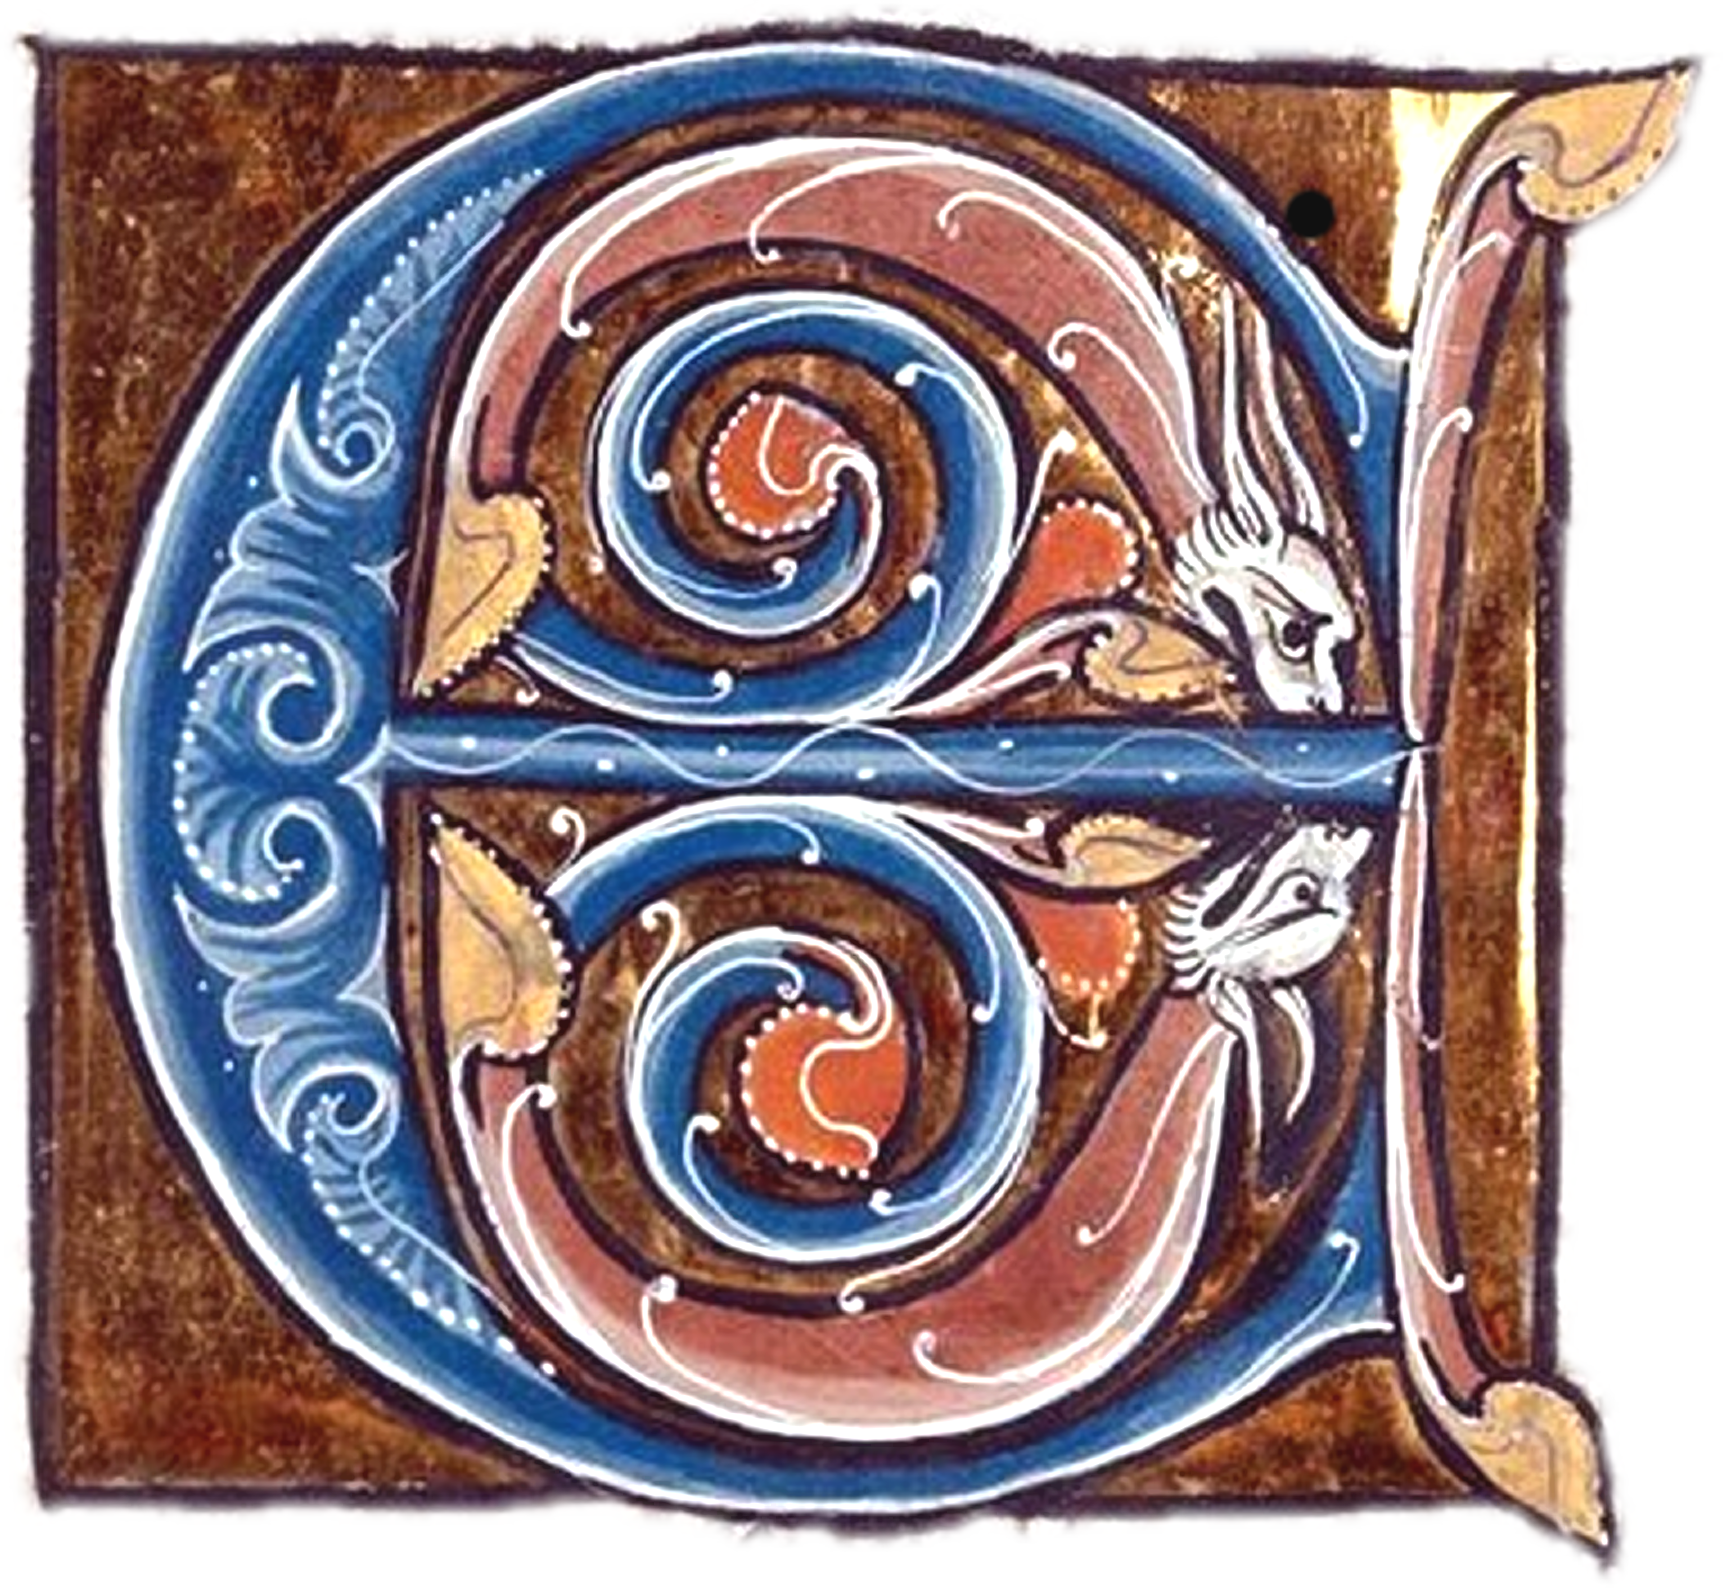
\includegraphics[height=12ex]{img/E0001}}}
\cantus{Introit}{CogitationesCordis}{Intr.}{5.}%
%}

\cantus{Graduel}{DulcisEtRectus}{Grad.}{1.}

\needspace{.2\paperheight}
\cantus{Alleluia}{TolliteIugum}{}{3.}

%\rubrica{Tempore Paschali :}

\cantus{Alleluia}{VeniteAdMe}{}{8.}

%\rubrica{Post Septuagesimam :}

\cantus{Trait}{Misericors}{Tract.}{2.}

%\needspace{.5\paperheight}
\cantus{Offertoire}{ImproperiumExspectavit}{Off.}{8.}

\cantus{Communion}{UnusMilitum}{Comm.}{7.}

%{\centering \textbf{Dominica IX. post Pentecosten}\par}

\bigskip

\cantus{Introit}{EcceDeus}{Intr.}{5.}

\cantus{Graduel}{DomineDominusNoster}{Grad.}{5.}

\cantus{Alleluia}{EripeMe}{}{2.}

\cantus{Offertoire}{IustitiaeDomini}{Off.}{4.}

\cantus{Communion}{QuiManducat}{Comm.}{6.}

%{\centering \textbf{Dominica I. post Pentecosten}\par}
\chead{Dominica I. post Pentecosten}

\bigskip

\cantus{Introit}{DomineInTuaMisericordia}{Intr.}{5.}

\cantus{Graduel}{EgoDixi}{Grad.}{5.}

\cantus{Alleluia}{VerbaMea}{}{2.}

\cantus{Offertoire}{IntendeVoci}{Off.}{5.}

\cantus{Communion}{NarraboOmnia}{Comm.}{2.}

%{\centering \textbf{Dominica III. post Epiphaniam}\par}
\chead{Dominica III. post Epiphaniam}

\bigskip

\cantus{Introit}{AdorateDeum}{Intr.}{7.}%

\cantus{Graduel}{TimebuntGentes}{Grad.}{5.}

\cantus{Alleluia}{DominusRegnavit_Exsultet}{}{8.}

\cantus{Offertoire}{DexteraDomini}{Off.}{2.}

\cantus{Communion}{MirabanturOmnes}{Comm.}{7.}

%{\centering \textbf{S. Luciæ\\ Virginis et Martyris}\par}
\chead{\rubrum Festa Decembris. 13.}

\bigskip

\cantus{Introit}{Dilexisti}{Intr.}{8.}

\cantus{Graduel}{Dilexisti}{Grad.}{8.}

\needspace{.3\paperheight}
\cantus{Alleluia}{DiffusaEst}{}{8.}

\needspace{.3\paperheight}
\cantus{Offertoire}{Afferentur_proximae}{Off.}{4.}

\needspace{.3\paperheight}
\cantus{Communion}{Principes}{Comm.}{1.}

%{\centering \textbf{S. Pauli Eremitae}\par}
\chead{\rubrum S. Pauli Eremitae}

\bigskip

\cantus{Introit}{IustusUtPalma}{Intr.}{1.}

\cantus{Graduel}{IustusUtPalma}{Grad.}{2.}

%\needspace{.3\paperheight}
\cantus{Alleluia}{IustusGerminabit}{}{1.}

%\needspace{.3\paperheight}
\cantus{Offertoire}{InVirtuteTua}{Off.}{6.}

\cantus{Communion}{Laetabitur}{Comm.}{5.}

%{\centering \textbf{Beatæ Mariæ Virginis\\ Matris Sanctæ Spei}\par}
\chead{\rubrum Festa Ianuarii. 17.}

\bigskip

{%
\gresetinitiallines{2}
\grechangedim{beforeinitialshift}{0pt}{scalable}
\grechangedim{afterinitialshift}{1ex}{scalable}
\greillumination{\raisebox{2ex}{
\includegraphics[width=6.5em]{G}}}
\cantus{Introit}{Astitit}{Intr.}{3.}%
}

\needspace{.1\paperheight}
\cantus{Graduel}{Mementote}{Grad.}{5.}

\cantus{Alleluia}{TuGloriaIerusalem}{}{7.}

\cantus{Offertoire}{ImmolaDeo}{Off.}{3.}

\cantus{Communion}{FasciculusMyrrhae}{Comm.}{8.}

%{\centering \textbf{S. Melanii Confessoris}\par}
\chead{\rubrum Festa Ianuarii. 19.}

\bigskip

\cantus{Introit}{Statuit}{Intr.}{1.}

\cantus{Graduel}{DominePraevenisti}{Grad.}{4.}

\cantus{Alleluia}{IuravitDominus}{}{1.}

\cantus{Offertoire}{VeritasMea}{Off.}{2.}

\cantus{Communion}{BeatusServus}{Comm.}{3.}

%{\centering \textbf{SS. Fabiani Papæ\\ et Sebastiani Mart.}\par}
\chead{\rubrum Festa Ianuarii. 20.}

\bigskip

\cantus{Introit}{IntretInConspectu}{Intr.}{4.}

\cantus{Graduel}{GloriosusDeus}{Grad.}{1.}

\needspace{.3\paperheight}
\cantus{Alleluia}{SanctiTui_Benedicent}{}{2.}

\cantus{Offertoire}{Laetamini}{Off.}{1.}

\cantus{Communion}{Multitudo_AdEum}{Comm.}{2.}

%{\centering \textbf{In Purificatione B.M.V.}\par}
\chead{\rubrum Festa Februarii. 2.}

\medskip

\cantus{Introit}{Suscepimus}{Intr.}{1.}

%\needspace{.5\paperheight}
\cantus{Graduel}{SuscepimusDeus}{Grad.}{5.}

%\needspace{.3\paperheight}
\cantus{Alleluia}{SenexPuerum}{}{1.}

\needspace{.3\paperheight}
\cantus{Trait}{NuncDimittis}{Tract.}{8.}

\needspace{.3\paperheight}
\cantus{Offertoire}{DiffusaEst}{Off.}{8.}

\needspace{.3\paperheight}
\cantus{Communion}{Responsum}{Comm.}{8.}

{\centering \textbf{S. Agathæ\\ Virginis et Martyris}\par}
\chead{\rubrum Festa Februarii. 5.}

\bigskip

\cantus{Introit}{Gaudeamus_Agathae}{Intr.}{1.}

\needspace{.2\paperheight}
{\tolerance=9999%
\pretolerance=9999%
\cantus{Graduel}{AdiuvabitEam}{Grad.}{5.}%
}

\needspace{.2\paperheight}
\cantus{Alleluia}{Loquebar}{}{2.}

\needspace{.2\paperheight}
\cantus{Trait}{QuiSeminant}{Tract.}{8.}

\needspace{.2\paperheight}
\cantus{Offertoire}{Afferentur_postEam}{Off.}{1.}

\needspace{.2\paperheight}
\cantus{Communion}{QuiMeDignatusEst}{Comm.}{6.}


%{\centering \textbf{In Apparitione B.M.V. Immaculatæ}\par}
\chead{\rubrum Festa Februarii. 11.}

\medskip

\cantus{Introit}{VidiCivitatem}{Intr.}{8.}

\needspace{.5\paperheight}
\cantus{Graduel}{FloresApparuerunt}{Grad.}{5.}

%\needspace{.3\paperheight}
\cantus{Alleluia}{OstendeMihi}{}{3.}

\cantus{Trait}{TuGloriaIerusalem}{Tract.}{8.}

%\needspace{.3\paperheight}
\cantus{Offertoire}{AveGratiaPlena}{Off.}{1.}

%\needspace{.3\paperheight}
\cantus{Communion}{VisitastiTerram}{Comm.}{1.}

%{\centering \textbf{In Cathedra S. Petri Apostoli}\par}
\chead{\rubrum Festa Februarii. 22.}

\bigskip

\cantus{Introit}{Statuit}{Intr.}{1.}

\needspace{.5\paperheight}
\cantus{Graduel}{ExaltentEum}{Grad.}{5.}

\needspace{.3\paperheight}
\cantus{Alleluia}{TuEsPetrus}{}{2.}

\cantus{Trait}{TuEsPetrus}{Tract.}{2.}

\needspace{.3\paperheight}
\cantus{Offertoire}{TuEsPetrus}{Off.}{1.}

\needspace{.3\paperheight}
\cantus{Communion}{TuEsPetrus}{Comm.}{6.}

%{\centering \textbf{SS. Ioannis et Pauli Martyrum}\par}
\chead{\rubrum Festa Iunii. 26.}

\bigskip

\cantus{Introit}{MultaeTribulationes}{Intr.}{2.}

\cantus{Graduel}{EcceQuamBonum}{Grad.}{1.}

\cantus{Alleluia}{HaecEstVera}{}{8.}

\cantus{Offertoire}{Gloriabuntur}{Off.}{6.}

\cantus{Communion}{EtSiCoram}{Comm.}{1.}

%{\centering \textbf{Beatæ Mariæ Virginis\\ de Perpetuo Succursu}\par}
\chead{\rubrum Festa Iunii. 27.}

\bigskip

{%
\gresetinitiallines{2}
\grechangedim{beforeinitialshift}{0pt}{scalable}
\grechangedim{afterinitialshift}{1ex}{scalable}
\greillumination{\raisebox{2ex}{
\includegraphics[width=3.5em]{G}}}
\cantus{Introit}{Gaudeamus_MariaeVirginis_lettrine}{Intr.}{1.}%
}

\needspace{.1\paperheight}
\cantus{Graduel}{TotaFormosa}{Grad.}{1.}

\cantus{Alleluia}{AveMaria}{}{2.}

\cantus{Offertoire}{RecordareVirgo}{Off.}{1.}

\cantus{Communion}{ReginaMundi}{Comm.}{1.}

%{\centering \textbf{Commemoratio Beatæ Mariæ Virginis\\ de Monte Carmelo}\par}
\chead{\rubrum Festa Iulii. 16.}

\bigskip

{%
\gresetinitiallines{2}
\grechangedim{beforeinitialshift}{0pt}{scalable}
\grechangedim{afterinitialshift}{0pt}{scalable}
\greillumination{\raisebox{1em}{
\includegraphics[width=10\cm]{G}}}
\cantus{Introit}{Gaudeamus_MariaeVirginis_lettrine}{Intr.}{1.}%
}

\needspace{.3\paperheight}
\cantus{Graduel}{Benedicta}{Grad.}{4.}

\cantus{Alleluia}{PerTeDeiGenetrix}{}{1.}

\cantus{Offertoire}{RecordareVirgo}{Off.}{1.}

\cantus{Communion}{ReginaMundi}{Comm.}{1.}

%{\centering \textbf{S. Iosephi de Cupertino Conf.}\par}
\chead{\rubrum Festa Septembris. 18.}

\bigskip

\cantus{Introit}{DilectioDei}{Intr.}{8.}

\needspace{.3\paperheight}
\cantus{Graduel}{DominePraevenisti}{Grad.}{4.}

\cantus{Alleluia}{OculusDei}{}{2.}

\cantus{Offertoire}{EgoAutem}{Off.}{2.}

\cantus{Communion}{EgoSumPauper}{Comm.}{8.}

%{\centering \textbf{Feria VI.\\Quatuor Temporum Septembris}\par}

\bigskip


\cantus{Introit}{LaeteturCor}{Intr.}{2.}

\cantus{Graduel}{ConvertereDomine}{Grad.}{5.}

\cantus{Offertoire}{BenedicAnimaMea}{Off.}{5.}

\cantus{Communion}{AuferAMe}{Comm.}{2.}

%{\centering \textbf{In Dedicatione\\ S. Michaëlis Archangeli}\par}
\chead{\rubrum Festa Septembris. 29.}

\bigskip

\cantus{Introit}{BenediciteDominum}{Intr.}{3.}

\needspace{.3\paperheight}
\cantus{Graduel}{BenediciteDominum}{Grad.}{3.}

\needspace{.3\paperheight}
\cantus{Alleluia}{SancteMichael}{}{8.}

\needspace{.3\paperheight}
\cantus{Offertoire}{StetitAngelus}{Off.}{1.}

\needspace{.3\paperheight}
\cantus{Communion}{BenediciteOmnesAngeli}{Comm.}{3.}

%{\centering \textbf{S. Melanii Confessoris}\par}
\chead{\rubrum Festa Ianuarii. 19.}

\bigskip

\cantus{Introit}{Statuit}{Intr.}{1.}

\cantus{Graduel}{DominePraevenisti}{Grad.}{4.}

\cantus{Alleluia}{IuravitDominus}{}{1.}

\cantus{Offertoire}{VeritasMea}{Off.}{2.}

\cantus{Communion}{BeatusServus}{Comm.}{3.}

%{\centering \textbf{Pretiosissimi Sanguinis D. N. Iesu Christi}\par}

\bigskip

%{%
%\gresetinitiallines{2}
%\greillumination{\raisebox{2ex}{\hspace{-1ex}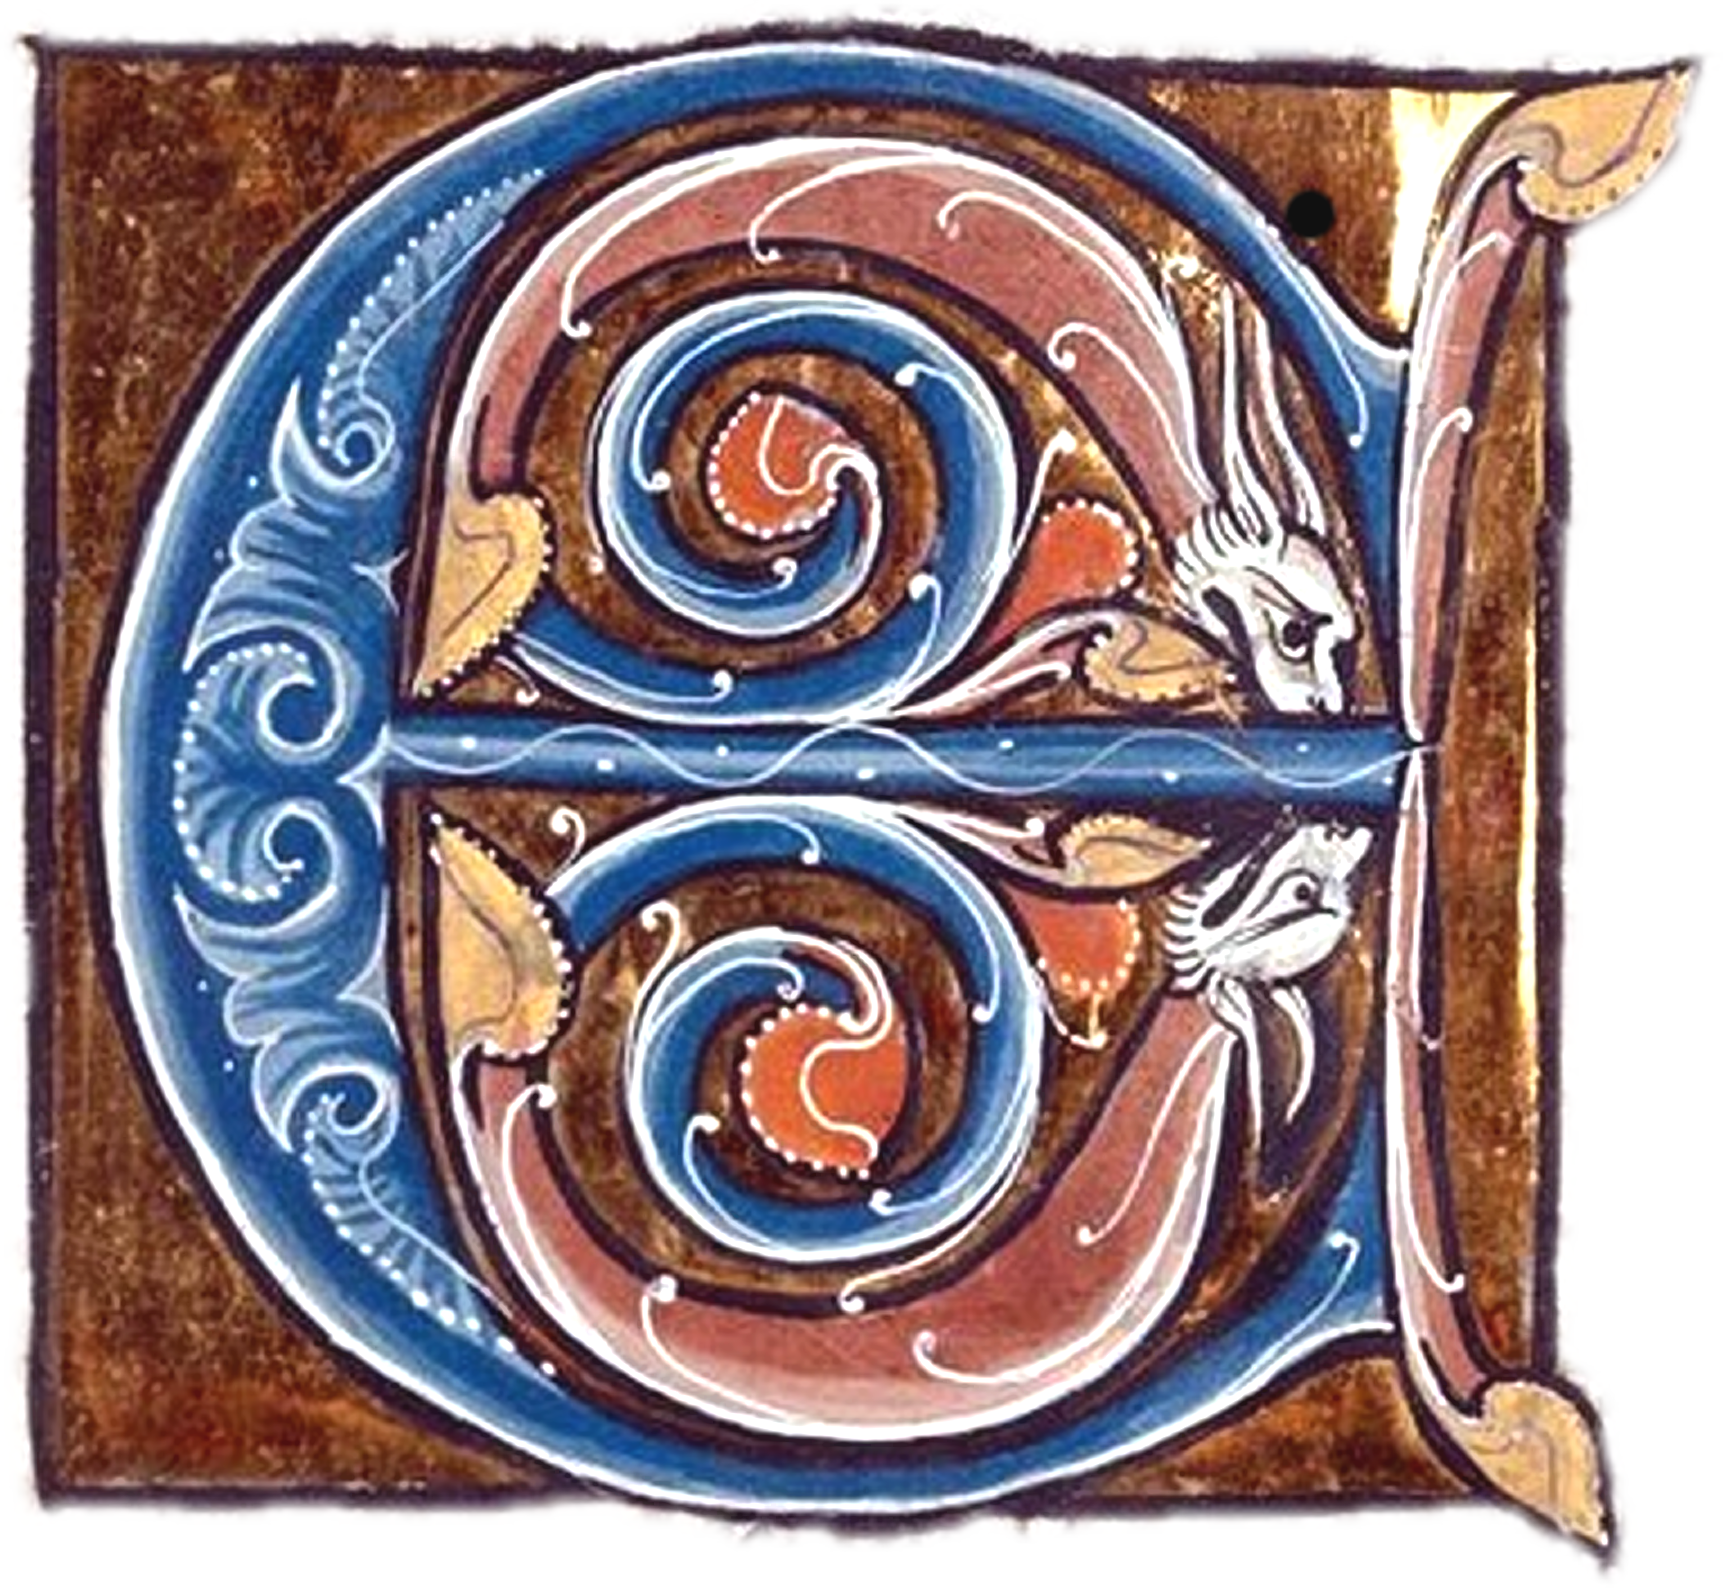
\includegraphics[height=12ex]{img/E0001}}}
\cantus{Introit}{RedemistiNos}{Intr.}{2.}%
%}

\cantus{Graduel}{HicEst}{Grad.}{5.}

\cantus{Alleluia}{VidimusStellam}{}{2.}

%\pagebreak
\cantus{Offertoire}{RegesTharsis}{Off.}{5.}

\cantus{Communion}{VidimusStellam}{Comm.}{4.}

%{\centering \textbf{Immaculati Cordis B. M. V.}\par}

\bigskip

%{%
%\gresetinitiallines{2}
%\greillumination{\raisebox{2ex}{\hspace{-1ex}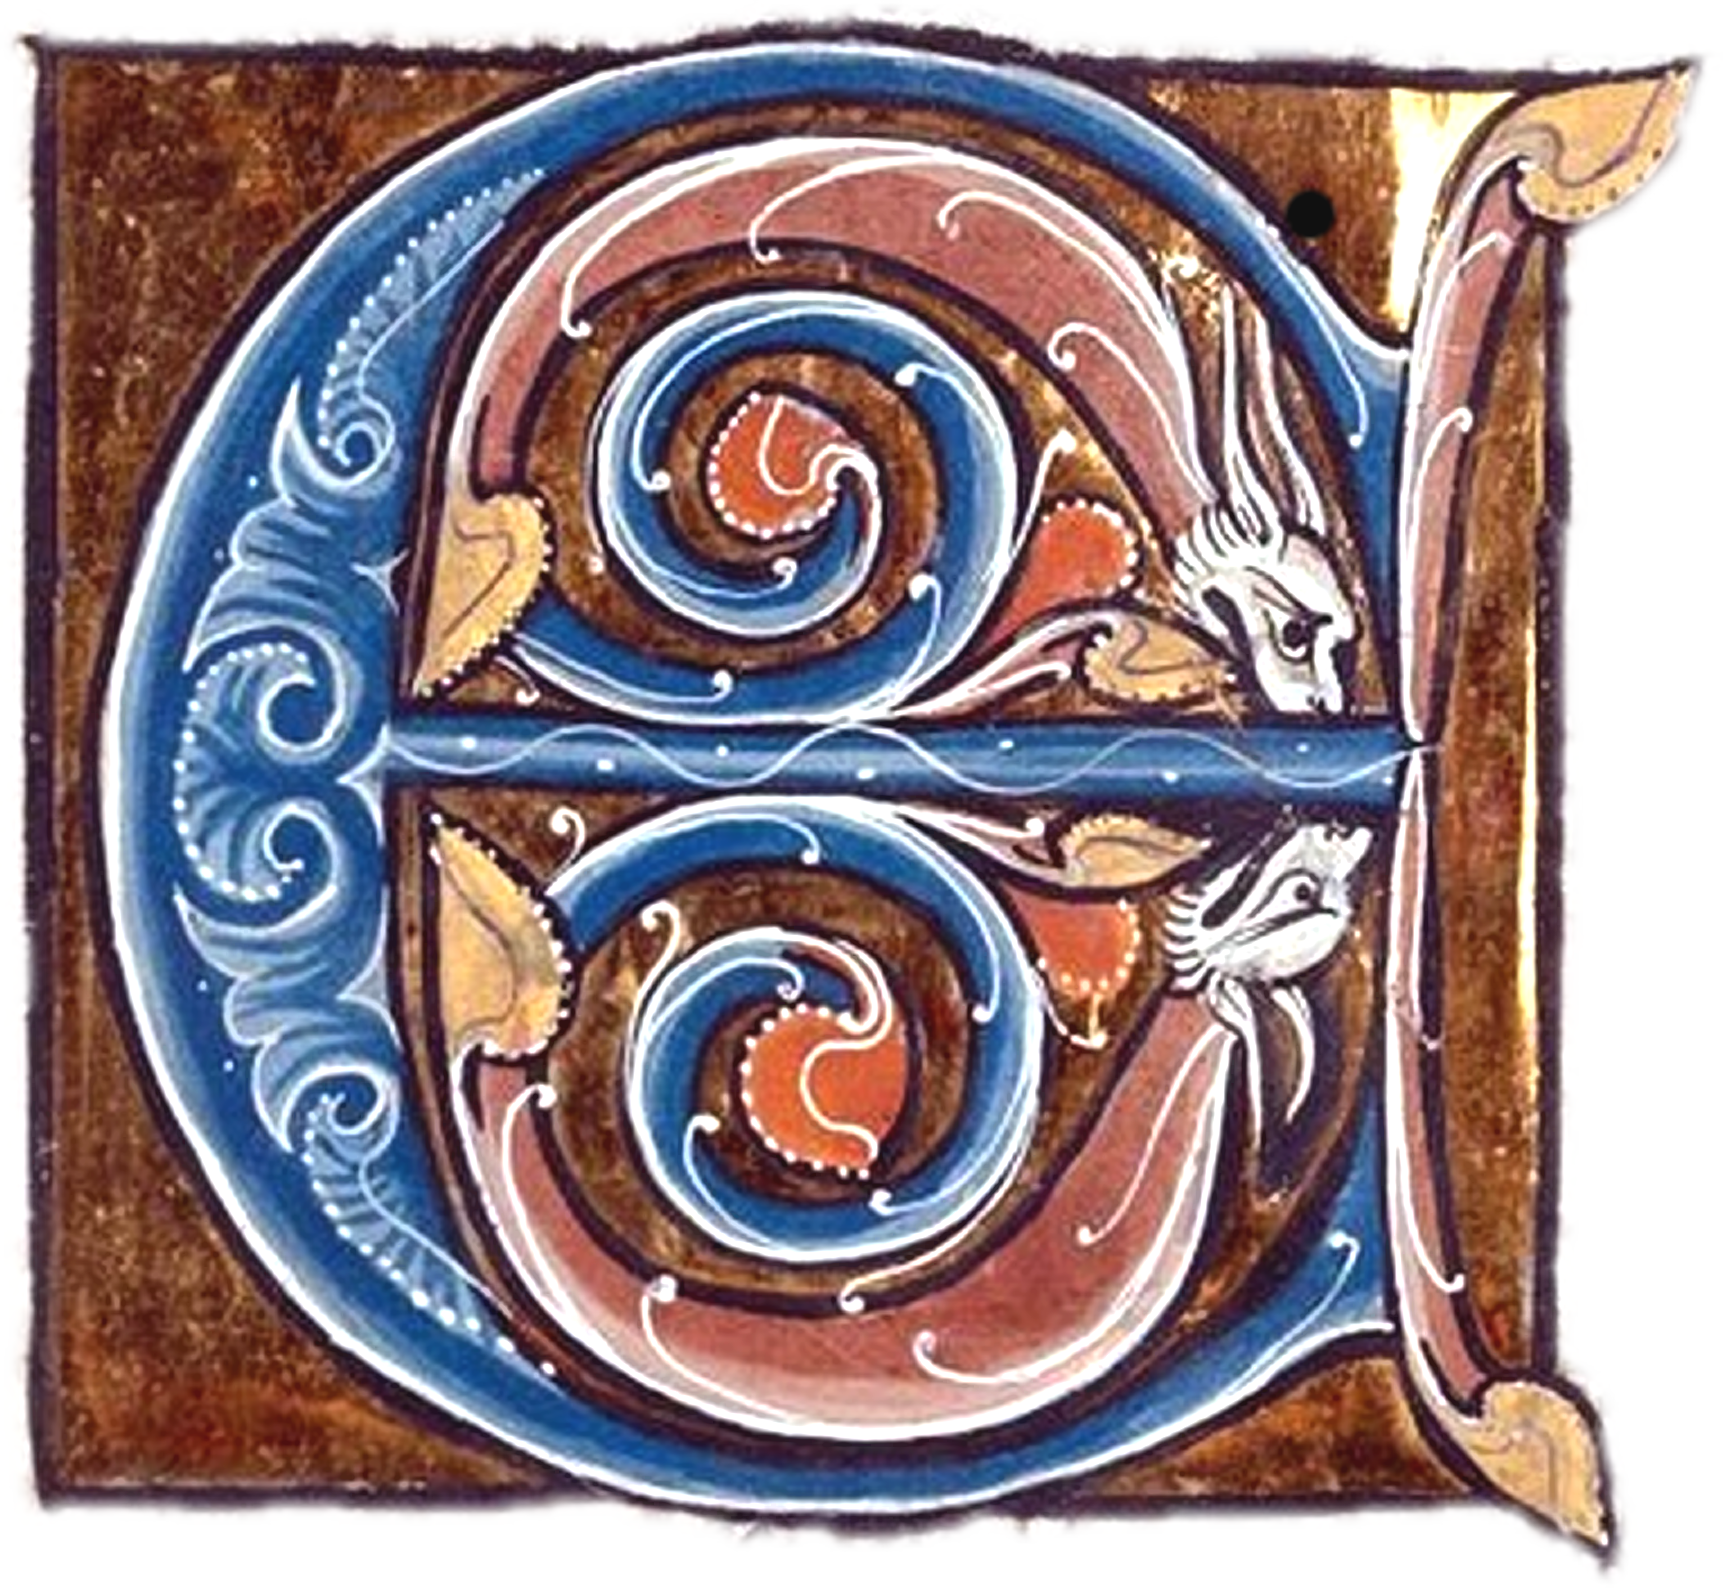
\includegraphics[height=12ex]{img/E0001}}}
\cantus{Introit}{Adeamus}{Intr.}{5.}%
%}

\cantus{Graduel}{Exsultabit}{Grad.}{2.}

\cantus{Alleluia}{Magnificat}{}{6.}

\rubrica{Tempore Paschali :}
\cantus{Alleluia}{BeatamMeDicent}{}{3.}

\rubrica{Post Septuagesimam :}
\cantus{Trait}{NuncErgo}{Tract.}{8.}


\pagebreak
\cantus{Offertoire}{Exsultavit}{Off.}{8.}

\pagebreak
\cantus{Communion}{DixitIesus}{Comm.}{4.}

%{\centering \textbf{In Epiphania Domini}\par}

\bigskip

{%
\gresetinitiallines{2}
\greillumination{\raisebox{2ex}{\hspace{-1ex}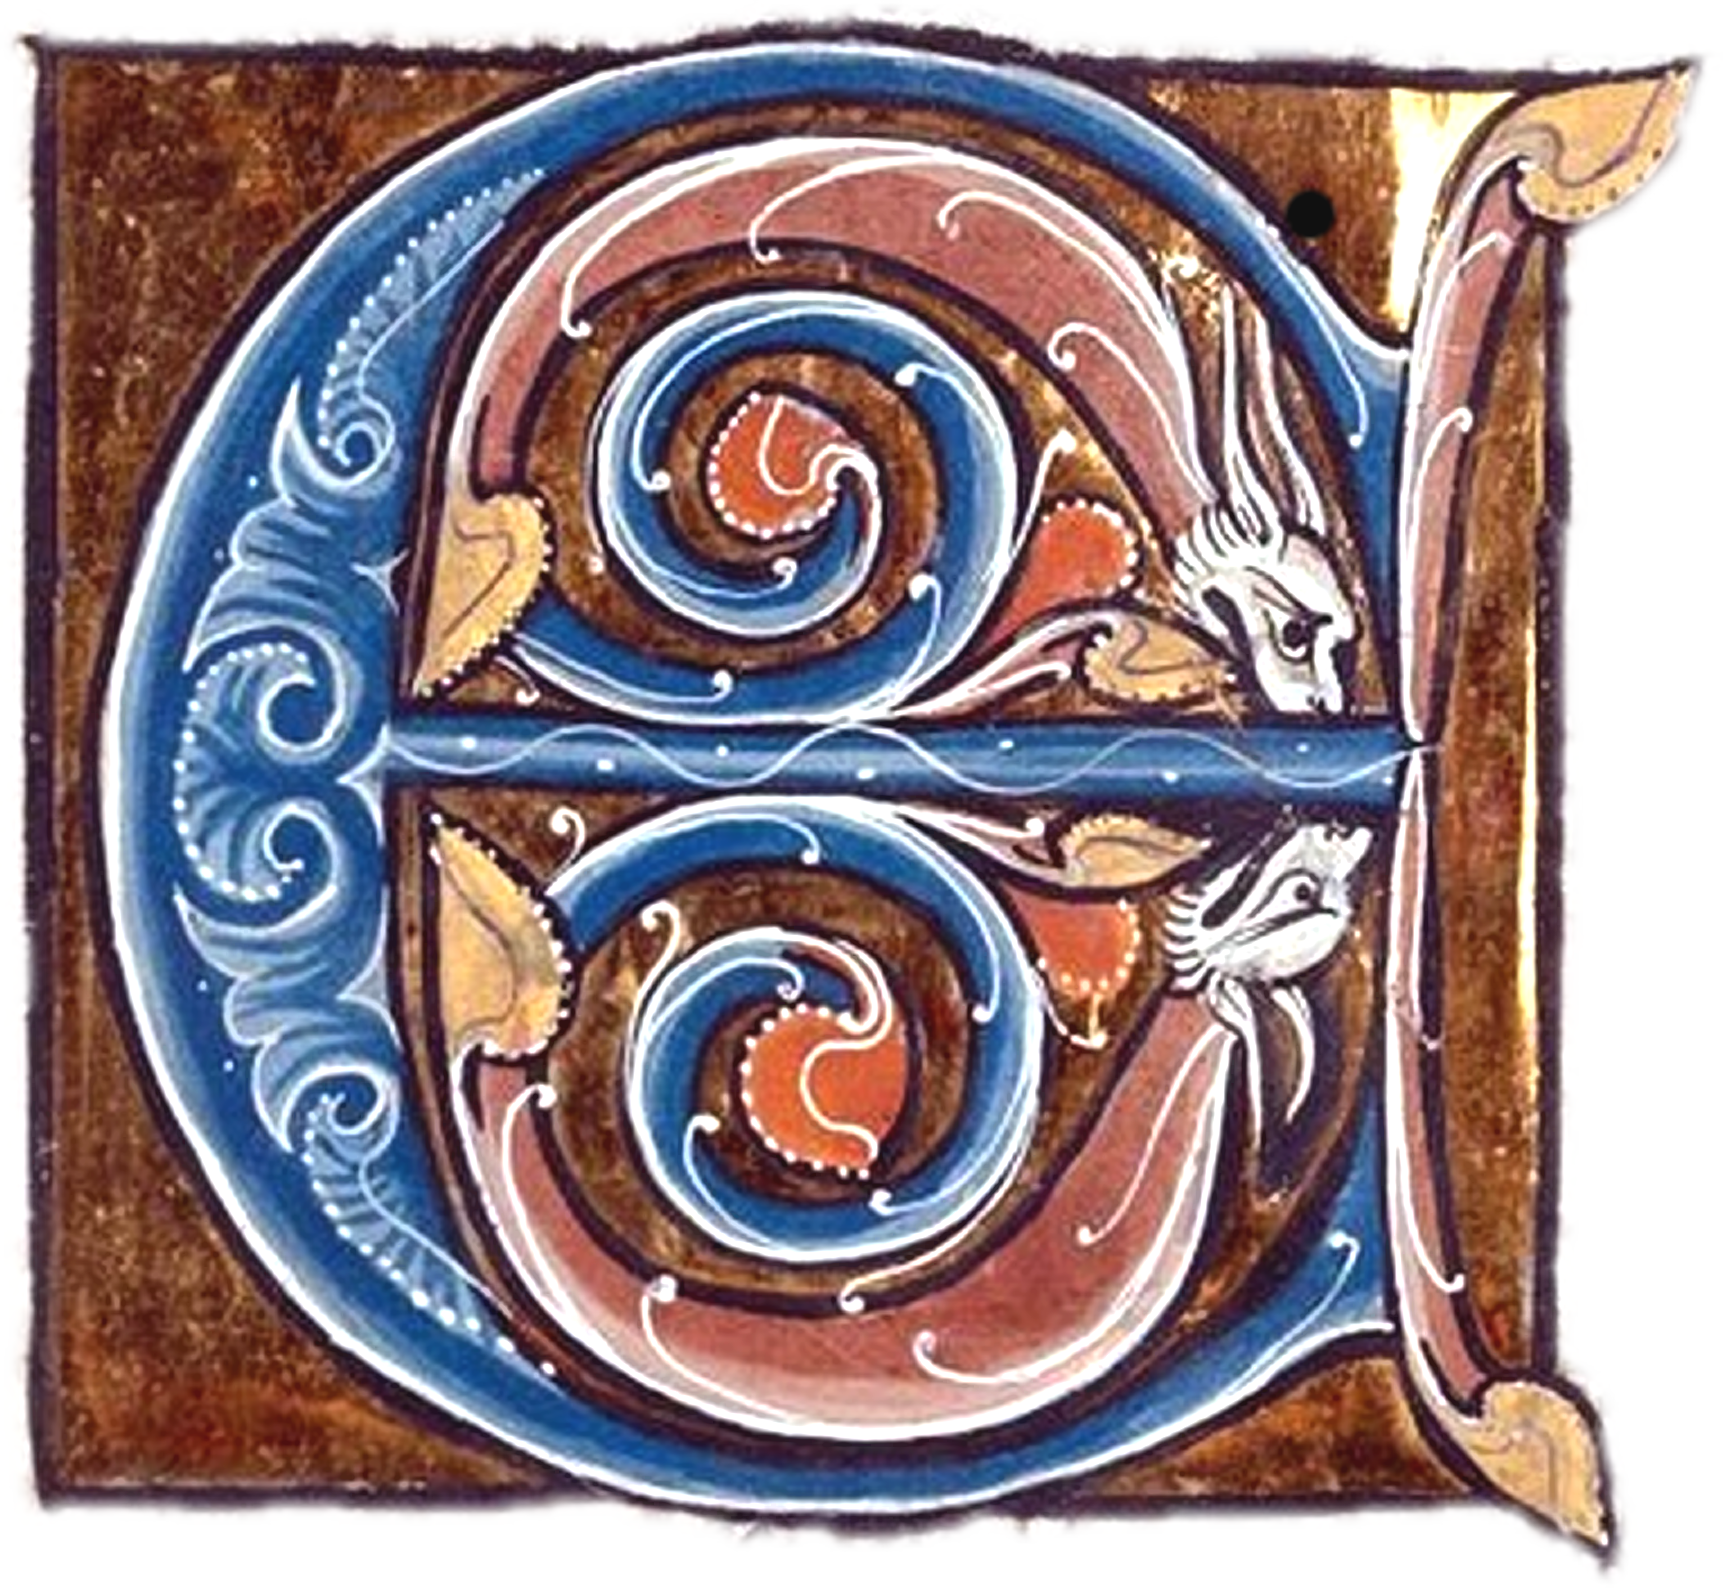
\includegraphics[height=12ex]{img/E0001}}}
\cantus{Introit}{EcceAdvenit}{Intr.}{2.}%
}

\cantus{Graduel}{OmnesDeSaba}{Grad.}{5.}

\cantus{Alleluia}{VidimusStellam}{}{2.}

%\pagebreak
\cantus{Offertoire}{RegesTharsis}{Off.}{5.}

\cantus{Communion}{VidimusStellam}{Comm.}{4.}

%{\centering \textbf{Commune Doctorum.}\par}
\chead{\rubrum Commune Doctorum.}

\bigskip

\cantus{Introit}{InMedio}{Intr.}{6.}

\needspace{.1\paperheight}
\cantus{Graduel}{OsIusti}{Grad.}{1.}

\needspace{.1\paperheight}
\cantus{Alleluia}{AmavitEum}{}{4.}

\needspace{.1\paperheight}
\cantus{Alleluia}{IustusGerminabit}{}{1.}

\needspace{.1\paperheight
\cantus{Trait}{BeatusVir}{Tract.}{8.}

\needspace{.1\paperheight}
\cantus{Offertoire}{IustusUtPalma}{Off.}{4.}

\needspace{.1\paperheight}
\cantus{Communion}{FidelisServus}{Comm.}{7.}

%{\centering \textbf{Commune plurimorum Martyrum \emph{extra T. P.}}\par}
\chead{\rubrum Commune plurimorum Martyrum}

\bigskip

\cantus{Introit}{IntretInConspectu}{Intr.}{4.}

\cantus{Graduel}{GloriosusDeus}{Grad.}{1.}

\needspace{.3\paperheight}
\cantus{Alleluia}{CorporaSanctorum}{}{2.}

\cantus{Trait}{QuiSeminant}{Tract.}{8.}

%\needspace{.3\paperheight}
\cantus{Offertoire}{MirabilisDeus}{Off.}{8.}

\cantus{Communion}{EtSiCoram}{Comm.}{1.}

%{\centering \textbf{Commune Confessoris\\non Pontificis. II.}\par}
\chead{\rubrum Comm. Conf. non Pontificis. II.}

\bigskip

\cantus{Introit}{IustusUtPalma}{Intr.}{1.}%

\cantus{Graduel}{OsIusti}{Grad.}{1.}

\needspace{.3\paperheight}
\cantus{Alleluia}{BeatusVirQuiTimet}{}{5.}

\needspace{.3\paperheight}
\cantus{Offertoire}{InVirtuteTua}{Off.}{6.}

\cantus{Communion}{AmenDicoVobisQuodVos}{Comm.}{1.}

%{\centering \textbf{Commune Confessoris\\non Pontificis. II.}\par}
\chead{\rubrum Comm. Conf. non Pontificis. II.}

\bigskip

\cantus{Introit}{IustusUtPalma}{Intr.}{1.}%

\cantus{Graduel}{OsIusti}{Grad.}{1.}

\needspace{.3\paperheight}
\cantus{Alleluia}{BeatusVirQuiTimet}{}{5.}

\needspace{.3\paperheight}
\cantus{Offertoire}{InVirtuteTua}{Off.}{6.}

\cantus{Communion}{AmenDicoVobisQuodVos}{Comm.}{1.}

%{\centering \textbf{Missa de Angelis.}\par}
\chead{\rubrum Missa de Angelis.}

\bigskip

\cantus{Introit}{BenediciteDominum}{Intr.}{3.}

\cantus{Graduel}{LaudateDominum}{Grad.}{3.}

\needspace{.3\paperheight}
\cantus{Alleluia}{InConspectu_DomineDeus}{}{4.}

\needspace{.3\paperheight}
\cantus{Offertoire}{StetitAngelus}{Off.}{1.}
\cantus{Communion}{Angeli}{Comm.}{2.}

%{\centering \textbf{Missa pro sponsis}\par}

\bigskip

\cantus{Introit}{DeusIsrael}{Intr.}{3.}

\cantus{Graduel}{UxorTua}{Grad.}{2.}

\cantus{Alleluia}{MittatVobis}{}{8.}

\cantus{Offertoire}{InTeSperavi}{Off.}{2.}

\cantus{Communion}{EcceSicBenedicetur}{Comm.}{6.}

%{\centering \textbf{Missa pro defunctis}\par}

\bigskip

\cantus{Requiem}{ExsultabuntDomino}{Ant.}{1. f.}
\cantus{Requiem}{Subvenite}{Resp.}{4.}
\cantus{Introit}{Requiem}{Intr}{6.}
\cantus{Requiem}{Kyrie}{}{}
\cantus{Graduel}{Requiem}{Grad.}{2.}
\cantus{Trait}{Absolve}{Tract.}{8.}
\cantus{Requiem}{DiesIrae}{Seq.}{1.}
\cantus{Offertoire}{DomineIesuChriste}{Off.}{2.}
\cantus{Kyriale}{Sanctus-XVIII}}{}                                                                            
\cantus{Requiem}{AgnusDei}{}{}                                                                                 
\cantus{Communion}{LuxAeterna}{Comm.}{8.}                                                                           
\cantus{Requiem}{LiberaMe}{Resp.}{1.}                                                                               
\cantus{Requiem}{KyrieEleison-absoute}{}{}                                                                             
\cantus{Requiem}{InParadisum}{Ant.}{6.}

%{\centering \textbf{Ordo sepeliendi parvulos}\par}

\bigskip

\cantus{Requiem}{SitNomenDomini}{Ant.}{2. D.}

\cantus{Requiem}{HicAccipiet}{Ant.}{6. F.}

\cantus{Requiem}{Iuvenes}{Ant.}{4. E.}

\cantus{Requiem}{BenediciteDominum}{Ant.}{7. a.}


\end{document}
